\chapter{Procesamiento de Imagen}
\label{cap_im}
\section{Introducción}

Este proceso busca analizar las páginas de libros escaneados por parte de OCRMX  a través de un análisis de los colores que componen las imágenes. Dado que la colección es de arte y principalmente se compone de  libros de pintura y escultura, entre otros,  creemos que es relevante que el usuario  pueda buscar por similitud en texto y en imágenes. 


Para ello, el proceso se descompone en tres partes:  la primera es identificar aquellas páginas que tienen una pintura dentro de la página; la segunda, analizar los colores   que  componen las pinturas  y tercera, identificar aquellas páginas con pinturas similares por la composición de sus colores.

El resultado final es un listado de todas las imágenes que tienen otra imagen similar, de acuerdo a su composición cromática, en formato XML, que permite hacer recomendaciones a aquellos que consultan el catálogo sobre otros libros que tienen imágenes similares.

Se probaron diferentes técnicas y métodos para poder conseguir cada uno de los subprocesos necesarios para alcanzar el objetivo. En las siguientes secciones se describe con mayor detalle los métodos para cada uno de los procesos para encontrar  imágenes similares.  En general se puede resumir en lo siguiente:

\begin{enumerate}
\item Definir una colección fija y reducida de colores y transformar los píxeles de cada imagen al color más cercano a esta colección.
\item Analizar cada página e identificar si la página tiene una imagen e identificar la composición cromática de la imagen.
\item Una reducción de las imágenes identificadas en el proceso anterior a una dimensión de 200 x 300, dado que la alta calidad de las originales hace muy complicado analizarlas en su forma inicial.
\item Construir de una matriz en donde las columnas representan cada uno de los colores definidos en el paso 1, cada renglón representa una imagen y cada cuadro de dicho renglón representa el conteo de píxeles en la imagen que pertenecen al color definido por la columna.
\item Encontrar imágenes similares a través del algoritmo de Local Sensitive Hashing(LSH) que permite de manera eficiente y rápida encontrar aquellas imágenes parecidas, tomando como medida de similitud la distancia coseno entre los vectores del conteo de colores.
\end{enumerate}

El diagrama de flujo de esta sección es el siguiente : 

\begin{figure}[H]
\centering
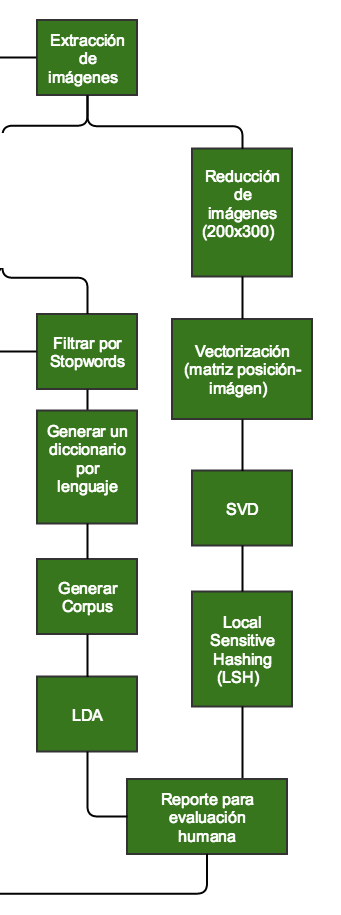
\includegraphics[width=0.3\textwidth]{Figures/pipeline_itam.png}
\caption{Pipeline procesamiento de imágenes}
\end{figure}


\section{Definir una colección fija y reducida de colores}

Para entender éste proceso y los subsecuentes se debe entender la forma por la cual las computadoras leen una imagen. Para esta acción existe un paradigma conocido como RGB, el cual descompone un color en tres capas: rojo, verde y azul, RGB por sus siglas en inglés. En cada una de estas capas existe un valor numérico que representa la intensidad de dicha capa, es decir la intensidad de azul, verde y rojo.  Cualquier color puede ser recreado como una combinación de estas (ver \cite{susstrunk1999standard}).


\begin{figure}[H]
\centering
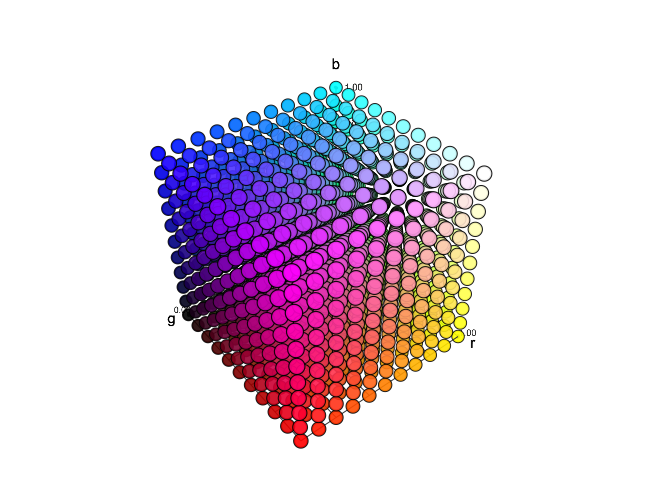
\includegraphics[width=1\textwidth]{Figures/cubo.png}
\caption{Espacio RGB}
\label{fig:cubo-rgb}
\end{figure}

Éste paradigma se ve reflejado en la figura \ref{fig:cubo-rgb}, en la cual se puede ver un cubo formado por distintos valores de rojo, verde y azul. Para este ejemplo, estos valores pueden ir del 0 al 1, representando este número la intensidad de cada capa, sin embargo, existen otras representaciones del paradigma en donde el valor puede ir de 0 a 256.

Respecto a las imágenes, estas se componen de píxeles, estos son pequeños puntos de colores que al aglomerarse forman la imagen. Toda imagen es entendida por la computadora como una composición de 3 matrices, una matriz con las intensidades de rojos, una de verdes y otra de azules, cada casilla de la matriz representa un píxel de la imagen cuyo color, como se vio en el párrafo anterior, se forma de la combinación de las tres capas.

Ahora, como se explicó antes, cada color se forma por la combinación de tres valores, en algunas ocasiones estos valores van del 0 al 1 y en otras del 0 al 256. Para nuestro caso, solo van del 0 al 1. Esto significa que el color que se forma de la combinación 0.935 en rojo, 0.267 en verde y 0.478 en azul es diferente del formado por 0.936, 0.268 y 0.479, respectivamente. Aunque visualmente una persona no pueda distinguir ambos colores,  la computadora los entiende como diferentes. Esto es relevante porque si uno de los objetivos es identificar los colores que se encuentran en la imagen, pequeñas variaciones en los dígitos harán que la computadora identifique millones de colores dentro de una imagen,  complicado cualquier tipo de análisis posterior. 

Para solucionar esta dificultad, se decidió limitar el número de colores que puede tomar un píxel, y convertir cada color de cada píxel a uno de los colores predefinidos. Esto reduce el número de posibles de colores que pueden existir en una imagen. Para realizar este proceso era importante desarrollar un método eficiente que permitiera de manera rápida hacer la transformación de cada píxel de las página. Si tomamos en cuenta que una página digitalizada tiene alrededor de 6,000,000 píxeles, que hay en promedio 200 páginas por libro y son más de 3,500 libros digitalizados, es fácil darse cuenta de lo tardado que podría ser el proceso en caso de no reducir el universo de colores.
 %%%%%%%%%%%%% Esto salió de mí %%%%%%%%%%%%%%%%%%%%%%%%%%%%%%%%%%%%%%%%%%%%%%%%%%%%%%%%%%%%%%%%%%%%%%%%%%%%%%%%

De esta forma se decidió, que la manera más rápida, sencilla y eficiente, era limitar el número de dígitos que podría tener los valores para la intensidad de las capas de rojo, verde y azul por medio de un redondeo a un dígito. Para clarificar, si volvemos al ejemplo donde un color se compone por 0.935, 0.267 y 0.478 de las capas respectivas, un redondeo a un dígito resultaría en 0.9, 0.3 y 0.5, u en otro caso más complicado, intensidades de 0.9836474, 0.6494334 y 0.3349854 se reduciría a 1, 0.6, 0.3. Con una sencilla función de redondear a un dígito, es posible redondear las tres matrices de la imagen de un solo golpe, lo que lo vuelve un método  rápido y efectivo.

Esto hace que exista una cantidad limitada de colores posibles en una imagen y existe una manera eficiente y rápida de transformar los colores a este universo. En concreto, los colores posibles que se pueden tener al hacer este redondeo son 1331, que son las combinaciones de 11 posibles dígitos (0, 0.1, 0.2, 0.3, 0.4, 0.5, 0.6, 0.7, 0.8, 0.9, 1) en tres capas, estos colores se pueden ver en la figura \ref{fig:colores-definidos}.  Y para una comparación de la alteración que sufrió  la imagen con esta transformación, véanse las figuras \ref{fig:paisaje-sin} y \ref{fig:paisaje-con}, antes y después de la transformación respectivamente. Se puede ver que la transformación no altera en gran medida la percepción visual de los colores y ayuda en gran medida a reducir la complejidad del problema.

\begin{figure}[H]
\centering
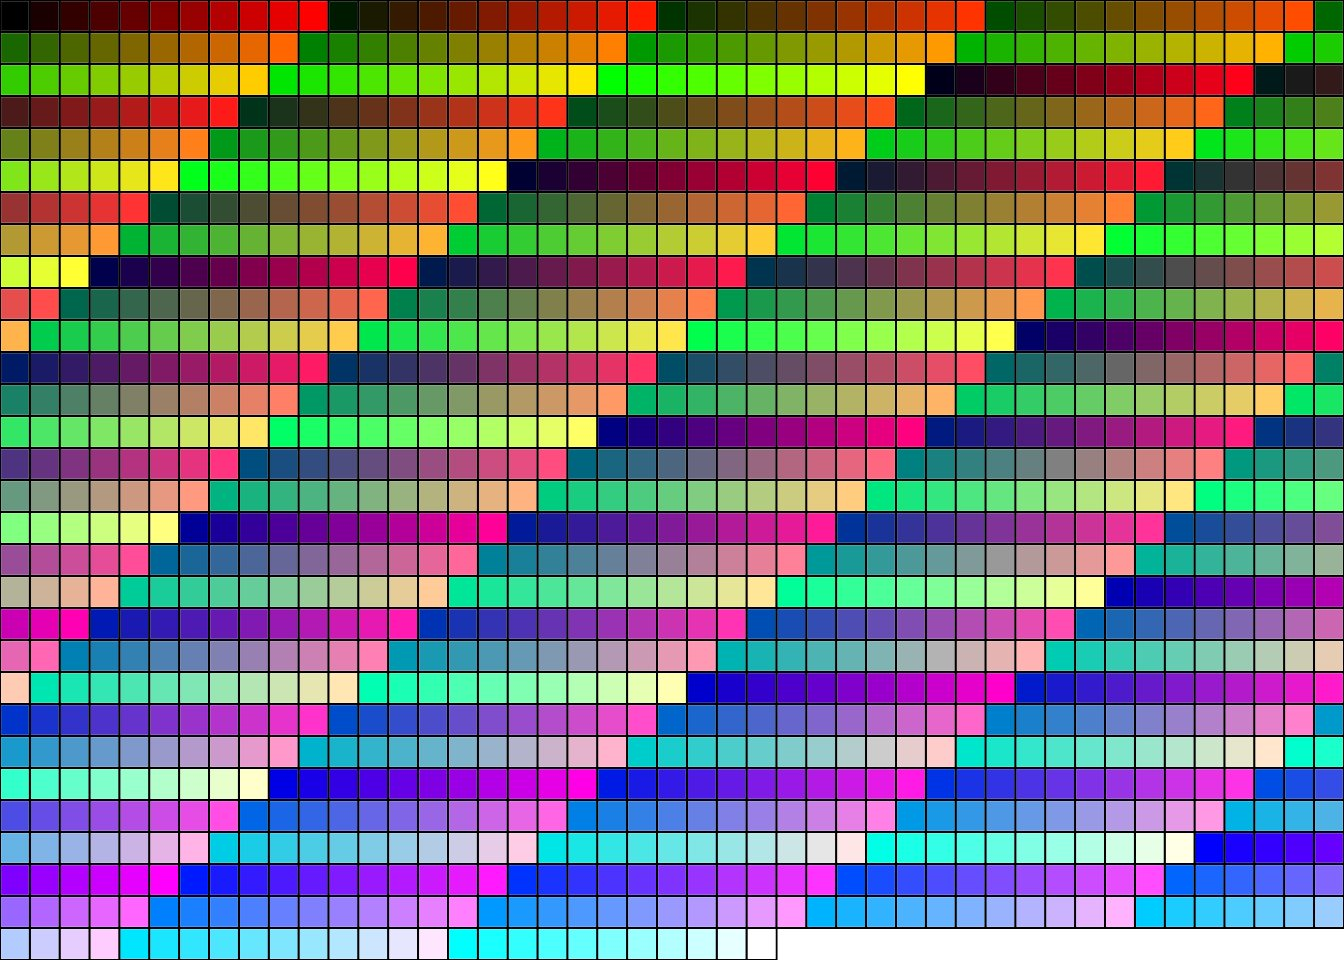
\includegraphics[width=0.8\textwidth]{Figures/colores_definidos.jpg}
\caption{Colores posibles en la imagen(1331).}
\label{fig:colores-definidos}
\end{figure}

\begin{figure}[H]
\centering
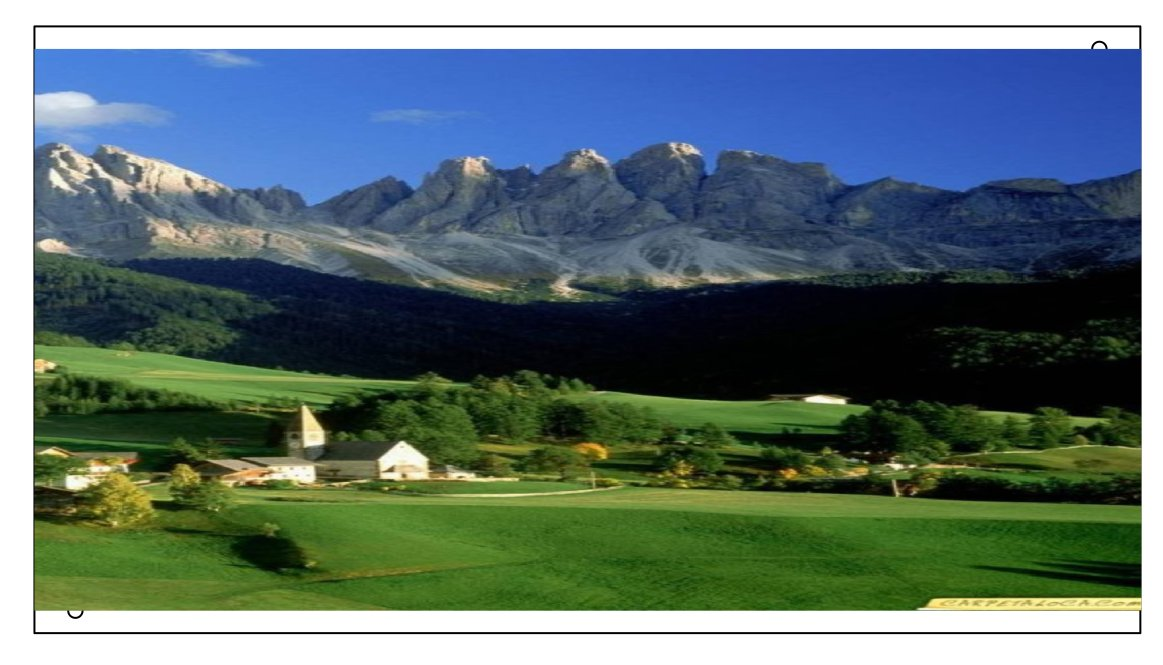
\includegraphics[width=0.8\textwidth]{Figures/paisaje_sin.jpg}
\caption{Paisaje sin alteración.}
\label{fig:paisaje-sin}
\end{figure}

\begin{figure}[H]
\centering
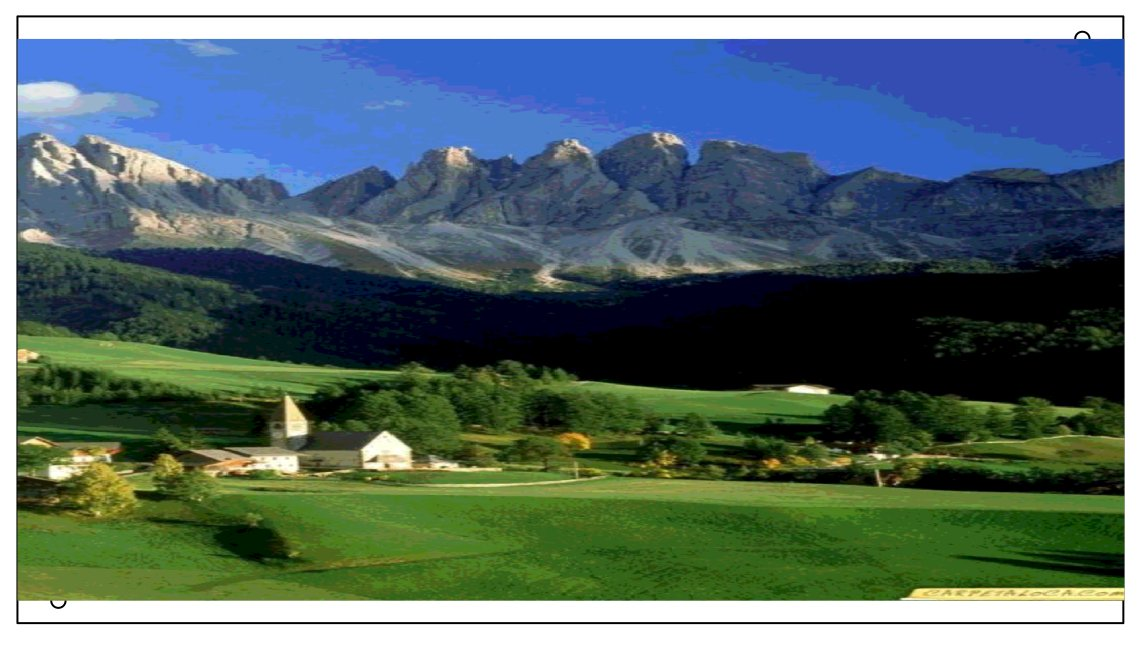
\includegraphics[width=0.8\textwidth]{Figures/paisaje_con.jpg}
\caption{Paisaje con reducción de colores.}
\label{fig:paisaje-con}
\end{figure}

\section{Identificar páginas con imágenes de colores}

El primer paso de éste proceso es  identificar  si una página contiene imágenes o no . Se realizaron pruebas para corroborar si la varianza de las matrices cromáticas de las imágenes eran de utilidad para dicho propósito. La colección de documentos contiene páginas en blanco, con texto monocromático, con texto multicromático y páginas con una o más imágenes, por lo que se espera que aquellas páginas que contienen imágenes tengan una mayor varianza que aquellas que solamente contienen texto. 


%%%%%%%%%%%%%%%%%%%%%%%%%%%%%%%%%%%%%%%%%%%%%%%%%%%%%%%%%%%%%%%%%%%%%%%%%%%%%%%%%%%%%%%%%%ME quedé revisando aquí 
 Para obtener la varianza de la imagen, no es necesario obtener esta con las tres matrices del RGB, es decir, la varianza de la página tendría que ser mayor incluso si la página estuviera en escala de grises. Es por ello que se decidió convertir las páginas a una escala de grises. Esto significa que ahora las imágenes no se componen de 3 capas de matrices, sino que ahora solo es una matriz, en la cual cada celda representa un píxel y el valor de dicha celda es la intensidad del negro, siendo 0 el blanco y el 1 el negro absoluto. Una vez transformadas las páginas en escalas de grises se saca su varianza, y si la varianza supera un número definido se considera que la página tiene una pintura dentro de la misma.

Para ilustrar mejor esta idea, véase la figura \ref{fig:varianza-sin} en donde estas páginas ya están en escala de grises y sus varianzas, de derecha a izquierda son 0.1074, 0.0515 y 0.0574. Se puede notar que existe una diferencia clara en las varianzas de la página de la izquierda respecto a la de la derecha, la cual solo contiene texto, sin embargo, la página de en medio tiene una varianza ligeramente menor que la de la derecha lo que indicaría que la varianza nos estaría ayudando para distinguir pinturas dentro de algunas páginas pero en otras fallaría.

\begin{figure}[H]
\centering
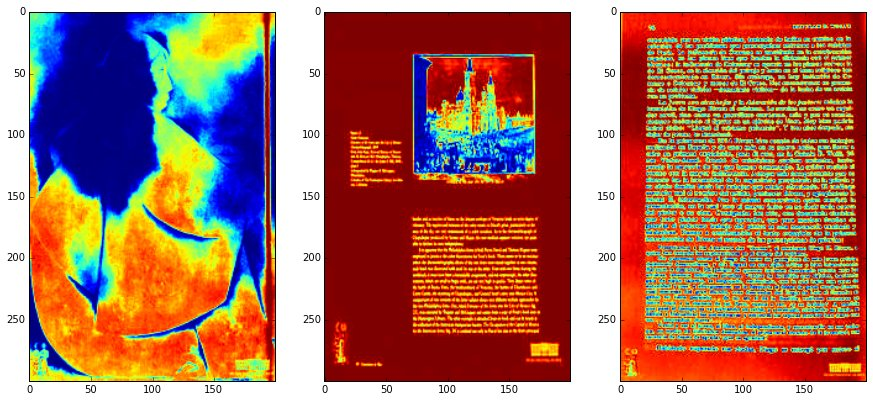
\includegraphics[width=1\textwidth]{Figures/prueba_varianza_1.jpg}
\caption{Identificación de imágenes sin filtro gaussiano}
\label{fig:varianza-sin}
\end{figure}

Para corregir este error, se usó un filtro gaussiano (ver \cite{burt1981fast}), que lo que hace es tomar un grupo de píxeles cercanos y promediarlos, esto hace que de alguna manera se difumina la imagen, como se puede ver en la figura \ref{fig:varianza-con}, pero al sacar la varianza ya con la transformación es mucho más útil para distinguir las páginas con contenido parecido a una pintura, ahora las varianzas son .0965, .0404 y .0146 respectivamente.

\begin{figure}[H]
\centering
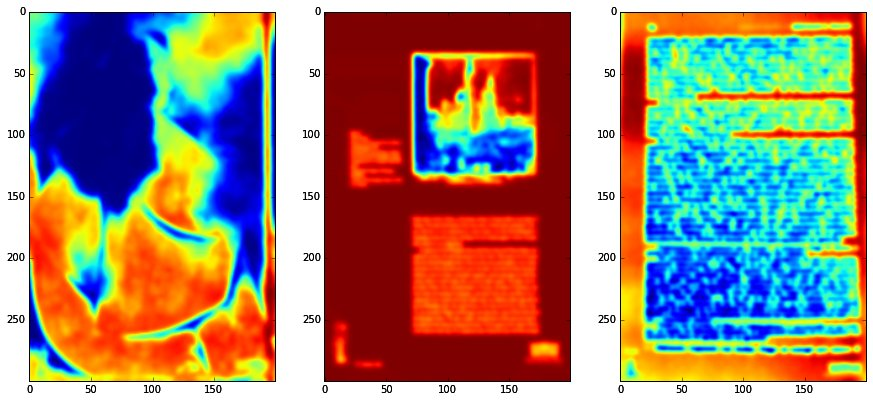
\includegraphics[width=1\textwidth]{Figures/prueba_varianza_2.jpg}
\caption{Identificación de imágenes con filtro gaussiano}
\label{fig:varianza-con}
\end{figure}

Avanzado el proyecto, con los resultados de las primeras pruebas, encontramos que existían muchísimos libros con imágenes en blanco y negro. En estos primeros resultados se encontraron muchas similitudes en imágenes en blanco y negro, aunque esto podría ser útil en alguna medida, el objetivo principal de este proyecto es sobre colores, por lo que decidimos enfocarnos en aquellas similitudes de imágenes a colores.

Para identificar las imágenes a colores se tuvo que idear un proceso por el cual al leer la página supiéramos si existen colores en esta o no, para después discriminar de nuestro análisis a las imágenes en blanco y negro. La manera más obvia para hacer esto es obteniendo la variedad de colores que existen en dicha imagen y si solo existen aquellos que van del blanco al negro, incluidos todas las escalas de grises, desecharlos y quedarnos con aquellas imágenes que tienen una mayor variedad de colores. Sin embargo, dado que son imágenes escaneadas, a pesar de que a simple vista las imágenes contenidas en las páginas fueran en blanco y negro, cuestiones de luz, basuritas microscópicas, entre otras cosas, hacían que incluso las páginas en blanco tuvieran una gran diversidad de colores.

Tal como usamos el filtro gaussiano para difuminar páginas previamente convertidas a escala de grises, se usó este filtro de nuevo para poder difuminar estas páginas pero ahora sin convertir a escala de grises, es decir se hizo el filtro sobre los tres canales del RGB.  Después de diversas pruebas para determinar cuál era la cantidad de colores diferentes necesarios para determinar si una imagen estuviera en color, se decidió el número de 100 colores diferentes como el límite. La figura \ref{fig:pruebas-colores} es parte de estas pruebas que se realizaron, estas ya tienen las 2 transformaciones mencionadas, una reducción de colores con el redondeo y el filtro gaussiano para los tres canales del RGB, en la parte superior de cada página se puede ver el número de colores diferentes que se encontraron en la página.

\begin{figure}[H]
\centering
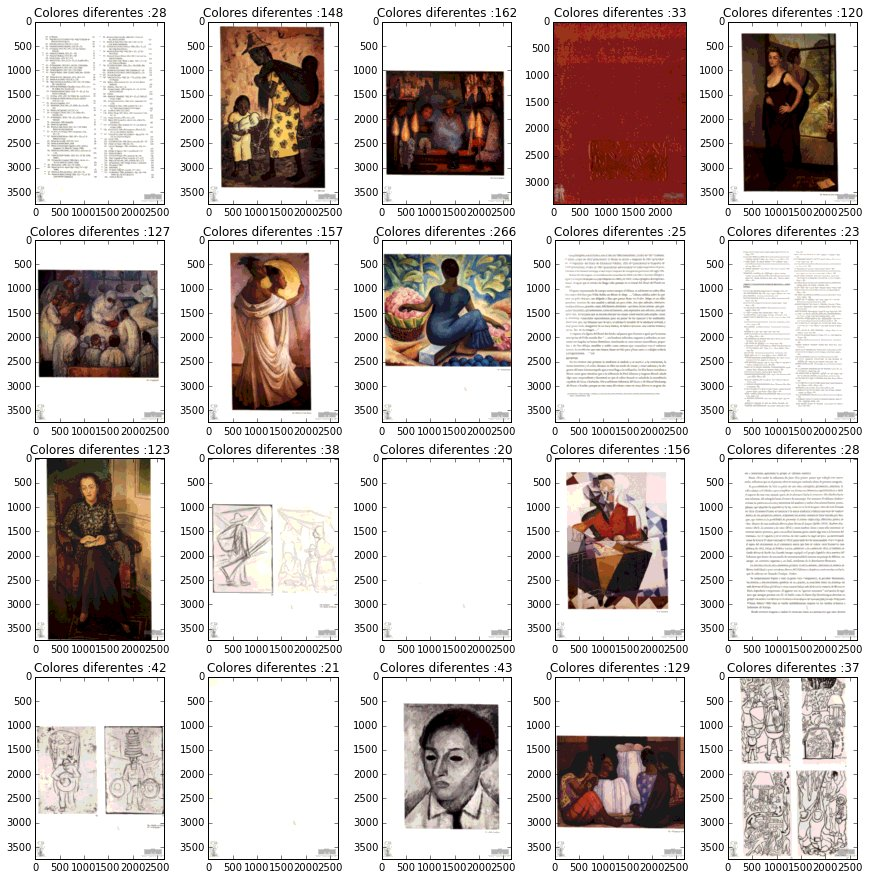
\includegraphics[width=1\textwidth]{Figures/identificar_colores.jpg}
\caption{Pruebas para determinar el número de colores mínimo}
\label{fig:pruebas-colores}
\end{figure}


Incluso, al realizar estas pruebas se percató que este procedimiento sirve para detectar qué páginas tienen imágenes dentro, por lo que el procedimiento de la varianza es reemplazado por este nuevo procedimiento de detección de color. Es decir, que el proceso de detección de colores  funciona a la vez para identificar imágenes porque entre más colores tenga la página mayor es la probabilidad de que sea por una imágen contenida en ella.

\section{Reducción de páginas a 200 x 300 píxeles}

La reducción de las imágenes obedece al hecho de que se tiene que realizar un conteo de los colores diferentes en cada página, este es diferente al que se realizó en el proceso pasado ya que en el anterior solo se buscaron los colores únicos, en este proceso se busca cuantos píxeles de cada uno de los 1331 colores definidos existen en la página. 

Las páginas escaneadas son de muy alta calidad, esta calidad es de alrededor de 2000 x 3000 píxeles, es decir que existen en la página cerca de 6 millones de píxeles, este número varía de pagina en pagina, pero en general no es muy distinto de este promedio. Dado lo anterior, hacer conteos sobre las páginas originales es muy tardado y ocupa mucha memoria RAM, por lo que para hacer el proceso más rápido y no desbordar la memoria se decidió hacer una reducción de aquellas páginas que se les detectó imágenes de colores. 

Este proceso se realiza con la librería de \texttt{Imagemagick} que corre sobre línea de comandos, particularmente se utilizó la función de  \texttt{mogrify} (ver \cite{still2005definitive}). Aunque la calidad de la imagen se pierde un poco, sigue siendo muy útil para realizar el análisis.

La figura \ref{fig:transformaciones} muestra el proceso por el cual se transformaron las imágenes, se debe mencionar que el filtro gaussiano no se incluye en esta transformación, ya que solo se utilizó para detectar imágenes pero la página no sufrió una modificación real. Cabe señalar que las originales se mantienen intactas, para aquellas que se realizan transformaciones permanentes se les hace una copia.

\begin{figure}[H]
\centering
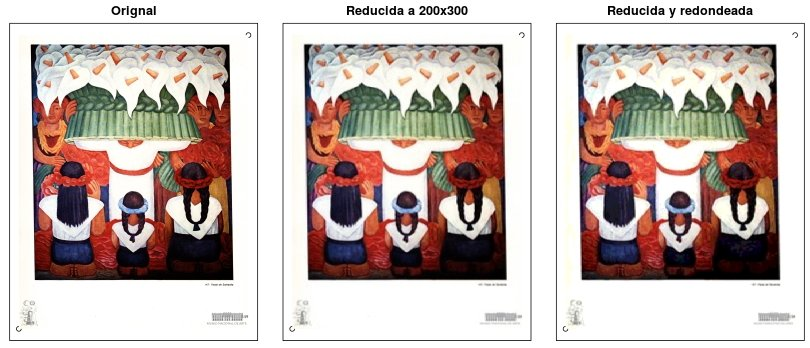
\includegraphics[width=1\textwidth]{Figures/transformaciones.jpg}
\caption{Proceso de modificación de imágenes, reducción y redondeo}
\label{fig:transformaciones}
\end{figure}

\section{Construcción de matriz de conteo de colores}

Como se mencionó en el apartado anterior, este proceso busca realizar un conteo de cada página de los colores que contiene, por lo que se abre cada página después de todos los procesos anteriores y se realiza un conteo de los colores, este conteo es transformado a un vector que es después consolidado a una matriz donde se están almacenando los conteos de todas las demás imágenes. Esta matriz tiene 1331 columnas que representan cada uno de los colores definidos, cada fila representa una imagen, y los datos en esta matriz son el número de píxeles que tiene cada imagen.

Se debe recordar que las imágenes que se analizan pertenecen a una página escaneada de un libro, por lo que es normal que la imagen no ocupe la página entera. 
Existe generalmente alrededor de la imagen un fondo blanco que puede hacer que el vector de colores esté muy cargado hacia este color, por otra parte, aunque se limitó el número de colores, todavía es suficientemente grande como para que existan diferentes tonalidades de un mismo color, es decir, que un color rosa de una flor,por ejemplo, va a tener diferentes tonalidades por los juegos de luces, lo que hace que se pulvericen los conteos de colores. Para tener más claro lo que se dijo veamos la figura \ref{fig:conteo-colores}, la cual es una página escaneada, si hacemos un conteo de sus colores y los representamos en una gráfica, se vería como la figura de en medio. 
El diámetro de las esferas representa la cantidad de píxeles que hay en dicho color, se puede notar que el color blanco es el preponderante, y que existe algunas esferas más chiquitas de colores diferentes, sin embargo se ven opacadas por el tamaño de los conteos de blanco. Si dejamos los vectores de conteo tal cual, va a ser afectado el algoritmo de similitud, ya que para determinar que tan parecidas son las imágenes toma en cuenta las proporciones de los colores, lo que resultaría en que todas las imágenes son parecidas ya que comparten en gran medida el blanco.

\begin{figure}[H]
\centering
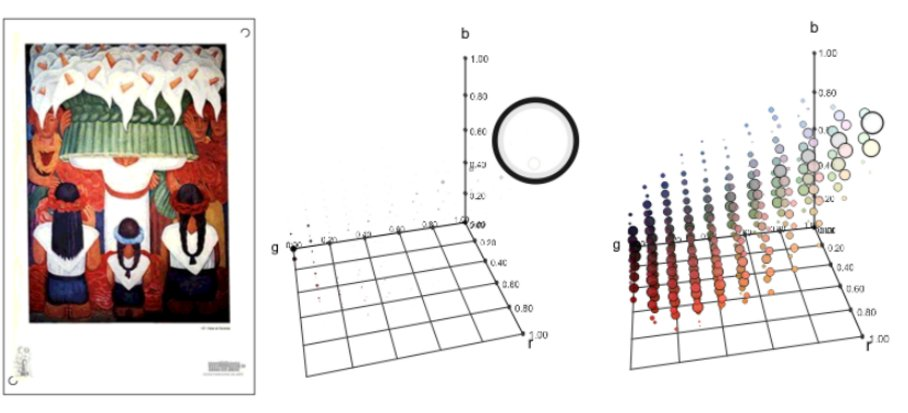
\includegraphics[width=1\textwidth]{Figures/conteo_colores.jpg}
\caption{Representación de conteo de colores}
\caption*{De lado izquierdo se encuentra la imagen escaneada después de reducción y redondeo de colores, en medio se encuentra la representación de conteo de colores en la dimensión RGB, de lado derecho está la representación del conteo pero después de sacar logaritmo natural.}
\label{fig:conteo-colores}
\end{figure}


Aunado a lo anterior, el fondo no debería contar dentro del conteo, ya que no es un color propio de la imagen, la solución ideal sería poder recortar el cuadro de la pintura para que el fondo no se incluyera dentro del conteo. Se realizaron pruebas con algoritmos de detección de esquinas para poder ver si era viable hacer este recorte de manera automática, este algoritmo no pudo identificar de manera clara las esquinas del cuadro ya que también detectaban esquinas dentro de la imagen, por lo que esta opción no se pudo seguir.

Para poder superar estas dificultades se utilizó en vez del conteo simple, el logaritmo del conteo, es decir, cada valor de la matriz se le aplicó el logaritmo natural para evitar que existieran valores tan disparatados, de esta forma el conteo de la imagen anterior ahora se vería como en la imagen de lado derecho de la figura \ref{fig:conteo-colores}. Se puede notar que el blanco deja de ocupar el lugar tan preponderante que tenía y que los colores tienen un mayor parecido con la imagen original.
 %%%%%%%%%%%%% Esto no lo tomé de nadie %%%%%%%%%%%%%%%%%%%%%%%%%%%%%%%%%%%%%%%%%%%%%%%%%%%%%%%%%%%%%%%%%%%%%%%%%%%%%%%%

\section{Encontrar imágenes similares}

Este es el proceso final, el que da como resultados las imágenes que se parecen. Una descripción más detallada del algoritmo de Local Sensitive Hashing lo podemos ver en un apartado más adelante, pero a grandes rasgos lo que busca es de manera rápida y eficiente determinar qué observaciones son parecidas de acuerdo a sus atributos. En el caso concreto de este proyecto una observación es una página de un libro con una imagen, los atributos de esta observación son el logaritmo del conteo de colores como se vio en el apartado anterior. La similitud la determinamos como la similitud coseno, que es una forma de calcular la similitud entre dos vectores (ver \cite{leskovec2014mining}).


Después de todos los procesos anteriores, se ejecutó el algoritmo de Local Sensitive Hashing y algunos de los resultados de este algoritmo de similitud son pares de imágenes que se encuentran en las figuras siguiente, las cuales tienen una similitud mayor al 90\% en sus colores. Es preciso mencionar que se debe juzgar su similitud no por el tema o las figuras de las pinturas, si no por la combinación de colores de las mismas.

\begin{figure}[H]
\centering
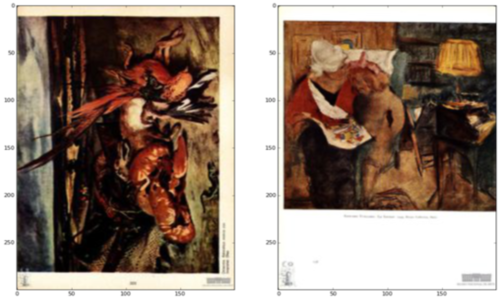
\includegraphics[width=0.8\textwidth]{Figures/similitud_1.png}
\caption{Par de imágenes similares 1}
\end{figure}

\begin{figure}[H]
\centering
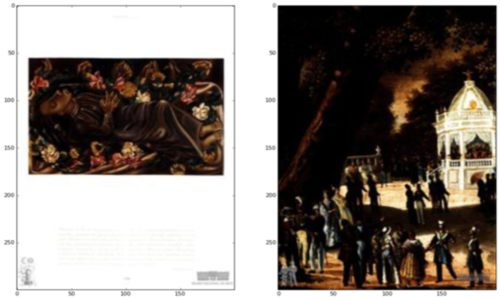
\includegraphics[width=0.8\textwidth]{Figures/similitud_2.png}
\caption{Par de imágenes similares 2}
\end{figure}

\begin{figure}[H]
\centering
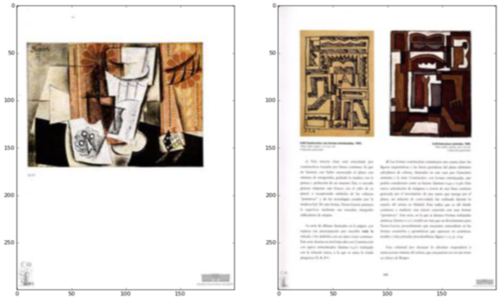
\includegraphics[width=0.8\textwidth]{Figures/similitud_3.png}
\caption{Par de imágenes similares 3}
\end{figure}

\begin{figure}[H]
\centering
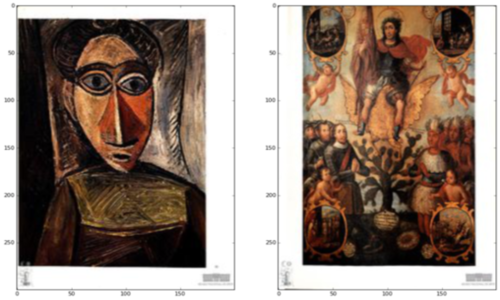
\includegraphics[width=0.8\textwidth]{Figures/similitud_4.png}
\caption{Par de imágenes similares 4}
\end{figure}

\begin{figure}[H]
\centering
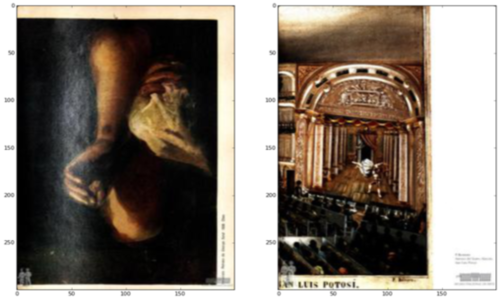
\includegraphics[width=0.8\textwidth]{Figures/similitud_5.png}
\caption{Par de imágenes similares 5}
\end{figure}

Para encontrar la similitud de imágenes se puede realizar una clasificación previa de las mismas, para poder agrupar aquellas imágenes que tienen una estructura de página similar. Es decir, aquellas páginas que tienen imágenes pequeñas dentro de ellas se distingan o se encuentren en un folder diferente de aquellas que tienen imágenes casi del tamaño de la página. Para realizar este proceso de agrupación se utilizaron k-medias, el cual busca agrupar aquellas observaciones que se encuentren más cercanas, siendo la medida de distancia la euclidiana.  Para realizar este proceso, cada imagen se debe convertir a una escala de grises, la matriz de la imagen que da como resultado es convertida en un vector que, dado la transformación previa a 200 x 300, tiene una longitud de 60,000. 

Esta matriz es la necesaria para ejecutar el algoritmo de k-medias, sin embargo, dado la longitud de los vectores y al gran número de páginas sobre las que tiene que calcular distancias, puede llegar a ser muy tardado este proceso, por lo que se decidió que para acelerar este proceso se podía hacer una reducción de dimensionalidad, que permitiera tener un menor número de variables sobre las cuales calcular las distancias. Para ello, se utilizó una descomposición de matrices llamada Singular Value Decomposition, SVD, quedándonos solo con las 8 componentes que capturaron en las pruebas el 40\% de la variabilidad de la matriz (ver \cite{leskovec2014mining}).


Ya con la reducción de las columnas de la matriz, es más rápido hacer el proceso de k-medias y se pueden crear el número de clusters que se desee. Los resultados pueden verse en las figuras \ref{fig:cluster2} y \ref{fig:cluster2}, que son imágenes que pertenecen a los clusters 1 y 2, respectivamente.

\begin{figure}[H]
\centering
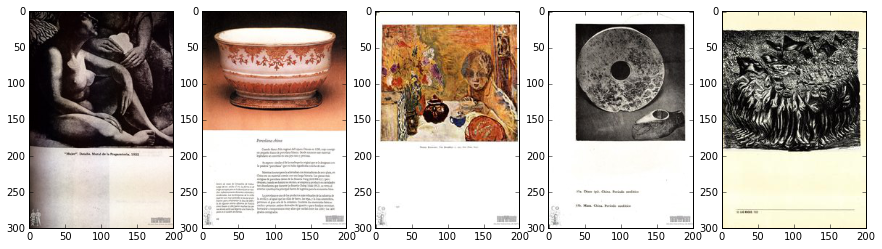
\includegraphics[width=1\textwidth]{Figures/cluster_1.png}
\caption{Muestra 1 de imágenes del cluster 1.}
\label{fig:cluster1}
\end{figure}

\begin{figure}[H]
\centering
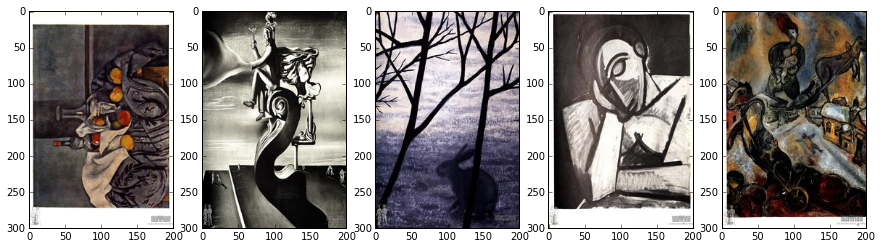
\includegraphics[width=1\textwidth]{Figures/cluster_2.png}
\caption{Muestra 2 de imágenes del cluster 1.}
\label{fig:cluster2}
\end{figure}

Este proceso de agrupación es opcional, y bien puede realizarse antes de correr el algoritmo de Local Sensitive Hashing para realizar similitud sólo sobre páginas con estructura de páginas similares, o bien puede dejarse de lado y correr sobre todas las páginas. Más detalles sobre estos algoritmos los veremos en las secciones siguientes.

\subsection{Filtro de extracción de imágenes}

La primera parte del pipeline consiste en crear un método para identificar las páginas que contienen imágenes, para ello se ha decidido transformar la imagen de color a escala de grises hacer un filtro de varianza. La idea consiste en que aquellas páginas que tienen sólo letras o están vacías tienden a ser más homogéneas, pero aquellas páginas con imágenes son más heterogéneas.





\subsection{ Singular Value Decomposition (SVD) \& K-Means}

Después de identificar para cada libro las páginas que tienen imágenes, copiamos dichos jpgs a una carpeta nueva y reducimos el tamaño del jpg a una estructura de 200 x 300 píxeles. Esto porque al momento de volver la imagen en vector, cada imagen puede tener un diferente número de píxeles oscilando entre los 2000 y los 2500 de ancho y entre 3000 y 3500 de alto, lo que imposibilitaría poder formar una matriz con todas las imágenes. Aunado a lo anterior, una matriz con un ancho de 2500 x 3500 , es decir una matriz con cerca de 8,750,000 columnas, sería intratable. 
Una técnica usual que se puede utilizar para este tipo de problemas
es la descomposición en valores singulares. En este caso, buscamos descomponer
una matriz $X$ de tamaño $nxm$ mediante


$$X=UDV^t$$

donde $U$ y $V$ son matrices ortogonales de tamaño $nxn$, $mxm$ y $D$ es una matriz
rectangular diagonal no negativa de tamaño $nxm$, con los componentes de su diagonal ordenados de forma decreciente (ver \cite{leskovec2014mining}). 

Resulta ser que esta descomposición siempre existe. Ahora supongamos que escogemos una $k$ chica, y definimos
- $U_k$ como la sub-matriz $nxk$  de $U$ donde seleccionamos las primeras $k$ columnas,
-  $V_k$ la sub-matriz $mxk$ de $V$ donde seleccionamos las primeras $k$ columnas,
- $D_k$ una matriz diagonal de $kxk$ (primeros $k$ renglones y $k$ columnas de $D$)

Entonces $X^k=U_k D_k V_k^t$ es \textbf{la matriz de rango} $k$ que minimiza
$$\sum (X_{ij} -X_{ij}^k )^2$$


Desde este punto de vista, esta descomposición parece resolver precisamente el
problema que queríamos: aproximar lo más cercano posible con una descomposición de matrices de rango bajo. En nuestro caso, podríamos tomar

\begin{itemize}
\item $U' = U_k D_k^{1/2}$
\item $V' = D_k^{1/2} V_k$
\end{itemize}

para obtener la descomposición que propusimos arriba. Con la transformación, nos quedaría una matriz con 6,000 columnas y filas como pinturas se encontraran en los libros.


En la colección de documentos hemos encontrado que las imágenes pueden venir de las siguientes maneras : 

\begin{itemize}
\item una imagen por página,
\item varias imágenes por página, 
\item mezcla de páginas y texto
\end{itemize}
Por el momento nos vamos a enfocar en las páginas que sólo tienen una imagen, para ello se realiza  un clustering, que nos sirva para formar grupos de páginas de acuerdo a la estructura. En clustering (o análisis de conglomerados) se busca agrupar “puntos” en “grupos”, de manera que puntos dentro de un cluster estén cercanos entre ellos, mientras que puntos en distintos clusters están a distancia más grande - todo esto de acuerdo a alguna medida de distancia.

K-medas es posiblemente el algoritmo más popular de segmentación, y  escala razonablemente bien a problemas medianos-grandes.

En k\-medias, un buen agrupamiento es uno en el que la variación dentro de los grupos
es chica. En primer lugar fijamos el número $K$ de grupos que buscamos. Supongamos entonces que $C_1\cup\cdots\cup C_K$ es una partición de los
datos, y sea $W(C_k)$ nuestra medida de variación dentro de los clusters. Entonces
buscaremos resolver

$$min_{C_1,\ldots, C_K} \sum_{k=1}^K W(C_k)$$ 

En general, este problema es imposible de resolver por enumeración, pues aún para un conjunto de datos chico con $K$ chica, el espacio de posibles particiones es inmenso.

Sin embargo, escogiendo mediadas $W$ particulares es posible construir algoritmos con desempeño razonable. En primer lugar, suponemos que $W(C)$ está dado por

$$W(C_k) =\frac{1}{|C_k|}\sum_{i,j\in C_k} ||x_i-x_j||^2,$$

es decir, la medida de variación dentro de los clusters es el promedio de distancias
euclídeas al cuadrado dentro del cluster. El problema

$$min_{C_1,\ldots, C_K} \sum_{k=1}^K \frac{1}{|C_k|}\sum_{i,j\in C_k} ||x_i-x_j||^2$$ 

todavía es demasiado difícil. Sin embargo, no es difícil demostrar (usando pitágoras) que

$$W(C_k)=2\sum_{i\in C_k} ||x_i-\bar{x}_k||^2,$$

donde $\bar{x}_k=\frac{1}{|C_k|}\sum_{i\in C_k} x_i$ es el centroide del grupo $C_k$.


y ahora notamos que si los $C_1,\ldots C_K$ están dados, entonces
tenemos que
$$\bar{x}_k = argmin_{m} \sum_{i\in C_k} ||x_i-m||^2,$$

(pues tenemos el teorema: el centroide es el punto con distancia euclidiana cuadrada promedio más baja a los elementos del grupo). Podemos entonces cambiar nuestro
problema original por el problema ampliado

$$min_{C_1,\ldots, C_K, m_1,\ldots, m_k} \sum_{k=1}^K \sum_{i\in C_k} ||x_i-m_k||^2$$ 

Vemos entonces que
\begin{enumerate}

\item  Si tenemos la asignación $C_1,\ldots C_K$, entonces podemos
encontrar las $m_1,\ldots, m_k$ calculando los centroides $m_k = \bar{x}_k$.
\item  Si tenemos los centroides $m_k$ fijos podemos resolver
$$min_{C_1,\ldots C_K} \sum_k \sum_{i\in C_j} ||x_i - m_k||^2$$
asignando cada punto a la $m_k$ más cercana.

\end{enumerate}

El primer paso es crear una matriz  con cada imagen en blanco y negro, en donde cada fila es una página con varianza alta y cada columna el deshilado de la matriz de la imagen en escala de grises, luego utilizaremos la descomposición de valores singulares para reducir la dimensionalidad y para posteriormente utilizar un  clustering con Kmeans. El número de Kmeans lo queremos pequeño pero suficientemente grande para separar bien las páginas, en las pruebas realizada un clustering con k=5 ha tenido un buen desempeño. A continuación se muestran los resultados. 


\subsection{ Local Sensitive Hashing (LSH)}

Para encontrar elementos similares en conjuntos de datos se necesita construir una medida de similitud adecuada, hacer eficiente éste cálculo y definir las reglas para encontrar grupos de objetos de similitud alta. A pesar de ser una técnica de minería de textos aplicamos este concepto para encontrar grupo de imágenes similares. 

Local Sensitive Hashing se concentra solamente en pares de documentos( en este caso imágenes) con alta probabilidad de ser similares ya que calcular todos los pares de similitud es poco factible. La idea central es  encontrar una manera de asignar las imágenes a una colección de cubetas de forma que imágenes con alta similitud caen en la misma cubeta. En este sentido \textbf{LSH} es una especie de clustering de datos (ver \cite{leskovec2014mining}).

En nuestro caso, la salida de LSH es una lista de pares de imágenes con alta
probabilidad de tener similitud alta.


Supongamos que tenemos un total de $k=br$ firmas de minhash\footnote{ minhashing es la reducción de dimensionalidad para estimar eficientemente similitud entre imágenes.} para una colección de imágenes.
Dividimos estas firmas en $b$ bandas (grupos) de $r$ minhashes cada una.

Observamos entonces que

- La probabilidad de que el minhash de una firma en particular coincida para un par de
documentos es $s$, que es el índice de jaccard entre los documentos. \footnote{El índice de jaccard es un estadístico para comparar la similitud de elementos, es definida como la intersección de los dos elementos dividida entre la unión (ver \cite{leskovec2014mining})}

- La probabilidad de que $r$ minhashes de una banda coincidan todos es $s^r$, pues las
funciones hash se seleccionan independientemente.
- La probabilidad de que al menos una de las bandas coincida totalmente es entonces
$1-(1-s^r)^b$ 

En consecuencia, la probabilidad de que al menos coincida una banda de minhashes en
función de la similitud se ve como sigue:

\begin{itemize}

\item Nótese que la probabilidad es 1/2 cuando $s=(1-0.5^{1/b})^{1/r}$
- La probabilidad es mayor a 0.90 cuando $s >(1-0.10^{(1/b)})^{1/r}$
\item Podemos entonces escoger $b$ y $t$ para capturar con alta probabilidad los niveles
de similitud que nos interesen, capturando tan pocos falsos negativos como deseemos.

\end{itemize}


Por ejemplo, si tenemos 20 bandas de tamaño 10, la probabilidad de coincidencia de al menos una banda es mayor a 0.90 cuando $s$ es más grande que 0.92

Una vez que tenemos nuestra matriz, donde cada imagen es una fila y en cada columna tenemos el conteo para cada uno de los colores, usamos Local Sensitive Hashing para determinar las imágenes que eran más similares de acuerdo a sus vectores de colores. Usamos 300 funciones hash, que simplemente son 300 vectores aleatorios de longitud 1,331, y agrupamos en 15 bandas de 20 hashes cada una. Luego del proceso de dividir las imágenes en distintas cubetas, de acuerdo a su similitud, calculamos la distancia coseno entre cada par que estuviera en la misma cubeta.


\section{Conclusión}

El proceso implementado en este trabajo tuvo como finalidad desarrollar una metodología que permitiera identificar imágenes dentro de las páginas y encontrar otras imágenes que fueran parecidas. Para ello se realizaron  4 procesos principales: 

\begin{enumerate}
\item Transformar los colores de cada página a una colección definida de colores.
\item Identificar si la imagen es a colores.
\item Una reducción de las imágenes identificadas. 
\item Construcción de una matriz de conteo de colores.
\item Encontrar similitud de imágenes.
\end{enumerate}

Esta descomposición del trabajo, no solo facilitó el abordar el problema sino que además permitió también programarlo de manera más sencilla en el esquema de \texttt{luigi}, lo que permitió realizar varios de estos procesos en paralelo y así reducir el tiempo de ejecución del proceso total.

La similitud que se encuentre en las imágenes sugeridas debe medirse en razón de los colores y no de los temas o formas tratadas en la pintura. No obstante lo anterior, creemos que esta similitud no es poca cosa ya que gran parte de las emociones que se transmiten en una pintura se debe a la combinación de colores que se emplearon.

\section{Problemas}

 En cada proceso se mencionó si existieron problemas. El principal problema  fue la dificultad 
 para procesar archivos pesados y  encontrar una forma de distinguir las páginas de colores de las que no. 
 
 A pesar de contar con una técnica robusta para distinguir  las páginas con imágenes no se pudo identificar el número de imágenes por página. Esto es relevante porque al momento de hacer conteo de colores, en páginas donde existen dos o más pinturas, se estaría  tomando el conteo de dos imágenes distintas para hacer su vector y al sugerir una imagen parecida se sugeriría  una imagen que se pareciera a la combinación de dos imágenes.

\section{Trabajo futuro}

Una forma de ampliar los resultados desarrollados en el presente trabajo, sería el poder contar con información acerca de las pinturas analizadas, información acerca de los autores, las fechas en las que se realzaron o los países en las que fueron pintadas. Esta información muchas veces se encuentra al pie de las pinturas y obtener esta información sería mucho más fácil si de entrada se supiera que en esa página existe una pintura.

Además, esta información permitiría hacer un análisis mucho más enriquecedor acerca de los colores en la pintura, permitiendo saber qué colores fueron los más utilizados en cada época o por cada autor.